\documentclass[border=8pt]{standalone}
\usepackage{tikz}
\usetikzlibrary{positioning,calc}
\definecolor{gA}{RGB}{72,116,158}   % G1
\definecolor{gB}{RGB}{86,156,104}   % G2
\definecolor{gC}{RGB}{198,148,76}   % G3
\definecolor{gD}{RGB}{142,108,176}  % G4
\definecolor{gE}{RGB}{120,120,120}  % G5
\begin{document}
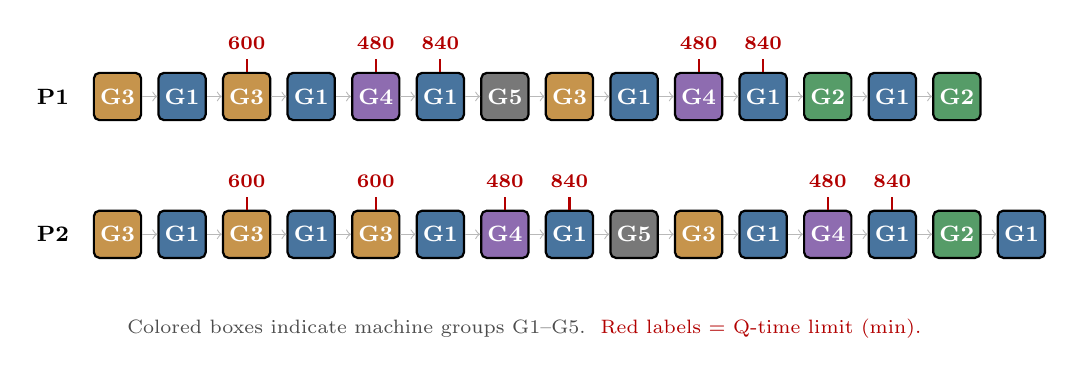
\begin{tikzpicture}[x=0.82cm,font=\footnotesize,
  op/.style={draw,thick,rounded corners=2pt,minimum width=0.6cm,minimum height=0.6cm,
             inner sep=0,align=center,text=white,font=\footnotesize\bfseries},
  qt/.style={red!70!black,font=\scriptsize\bfseries}]

  % ---- P1 : 14 operations ----
  \node at (0,0) {\bfseries P1};
  \foreach \g/\c [count=\i] in
    {G3/gC,G1/gA,G3/gC,G1/gA,G4/gD,G1/gA,G5/gE,G3/gC,G1/gA,G4/gD,G1/gA,G2/gB,G1/gA,G2/gB}
    \node[op,fill=\c] (p1-\i) at (\i,0) {\g};
  \foreach \i [evaluate=\i as \j using int(\i+1)] in {1,...,13}
    \draw[->,gray!55] (p1-\i)--(p1-\j);
  \foreach \i/\v in {3/600,5/480,6/840,10/480,11/840}{
    \draw[red!70!black,thick] (p1-\i.north)--++(0,0.16);
    \node[qt,above=0.16cm of p1-\i]{\v};}

  % ---- P2 : 15 operations ----
  \node at (0,-1.75) {\bfseries P2};
  \foreach \g/\c [count=\i] in
    {G3/gC,G1/gA,G3/gC,G1/gA,G3/gC,G1/gA,G4/gD,G1/gA,G5/gE,G3/gC,G1/gA,G4/gD,G1/gA,G2/gB,G1/gA}
    \node[op,fill=\c] (p2-\i) at (\i,-1.75) {\g};
  \foreach \i [evaluate=\i as \j using int(\i+1)] in {1,...,14}
    \draw[->,gray!55] (p2-\i)--(p2-\j);
  \foreach \i/\v in {3/600,5/600,7/480,8/840,12/480,13/840}{
    \draw[red!70!black,thick] (p2-\i.north)--++(0,0.16);
    \node[qt,above=0.16cm of p2-\i]{\v};}


  \node[align=left,anchor=west,font=\scriptsize,text=black!70] at (1,-2.95)
    {Colored boxes indicate machine groups G1--G5.\ \ \textcolor{red!70!black}{Red labels = Q-time limit (min).}};

\end{tikzpicture}
\end{document}
